\documentclass[tikz,convert={density=150,size=600,outext=.png}]{standalone}
\usetikzlibrary{shapes, calc, arrows, fit, positioning, decorations, patterns, decorations.pathreplacing, chains, snakes}

\begin{document}
  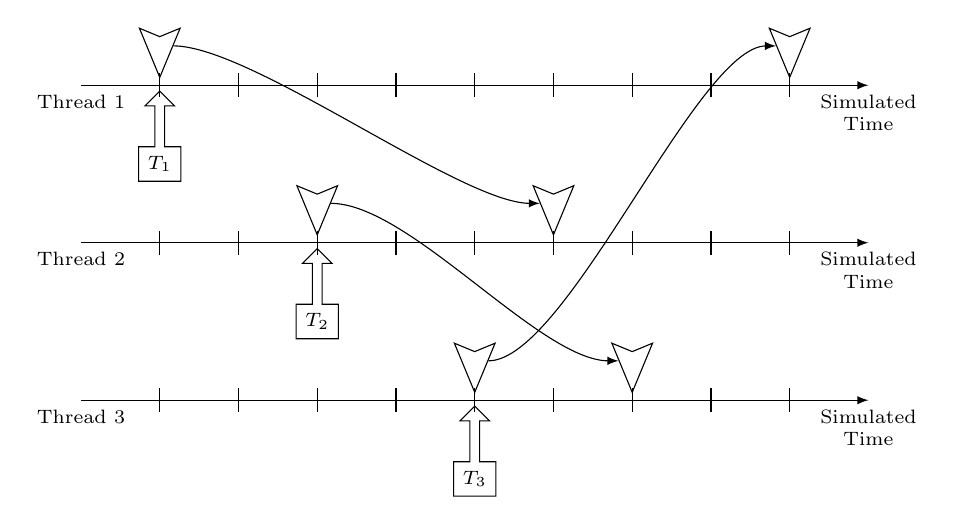
\begin{tikzpicture}[>=latex, font=\scriptsize]
    \draw[->] (0,0) -- (10,0)
      node[pos=1, below, align=center] (sim-time1) {Simulated\\Time}
      node[pos=0., below] {Thread 1};
    \foreach \x in { 1, 2, 3, 4, 5, 6, 7, 8, 9} { 
        \draw (\x,-0.15) -- (\x,0.15) node (tick\x) {};
    };
    \node[draw, arrow box, arrow box arrows={north:.7cm}] at (1, -1) {$T_1$};
    \node[shape=dart, draw, shape border rotate=270 ] at (1, 0.5)  (ev11) {};
    
    \draw[->] (0,-2) -- (10,-2)
      node[pos=1, below, align=center] (sim-time2) {Simulated\\Time}
      node[pos=0., below] {Thread 2};
    \foreach \x in { 1, 2, 3, 4, 5, 6, 7, 8, 9} { 
        \draw (\x,-2.15) -- (\x,-1.85) node (tick\x) {};
    };
    \node[draw, arrow box, arrow box arrows={north:.7cm}] at (3, -3) {$T_2$};
    \node[shape=dart, draw, shape border rotate=270 ] at (3, -1.5)  (ev21) {};
   
    \draw[->] (0,-4) -- (10,-4)
      node[pos=1, below, align=center] (sim-time3) {Simulated\\Time}
      node[pos=0., below] {Thread 3};
    \foreach \x in { 1, 2, 3, 4, 5, 6, 7, 8, 9} { 
        \draw (\x,-4.15) -- (\x,-3.85) node (tick\x) {};
    };
    \node[draw, arrow box, arrow box arrows={north:.7cm}] at (5, -5) {$T_3$};
    \node[shape=dart, draw, shape border rotate=270 ] at (5, -3.5)  (ev31) {};
    
    \node[shape=dart, draw, shape border rotate=270 ] at (9, 0.5)  (ev12) {};
    \node[shape=dart, draw, shape border rotate=270 ] at (6, -1.5)  (ev22) {};
    \node[shape=dart, draw, shape border rotate=270 ] at (7, -3.5)  (ev32) {};
    
    \draw[->] (ev11.east) .. controls +(1,0) and +(-1,0) .. (ev22.west);
    \draw[->] (ev21.east) .. controls +(1,0) and +(-1,0) .. (ev32.west);
    \draw[->] (ev31.east) .. controls +(1,0) and +(-1,0) .. (ev12.west);
  \end{tikzpicture}
\end{document}
